% !Mode:: "TeX:UTF-8"

\chapter{项目特色}
\begin{enumerate}
\item
\begin{figure}[htbp]
    \centering
    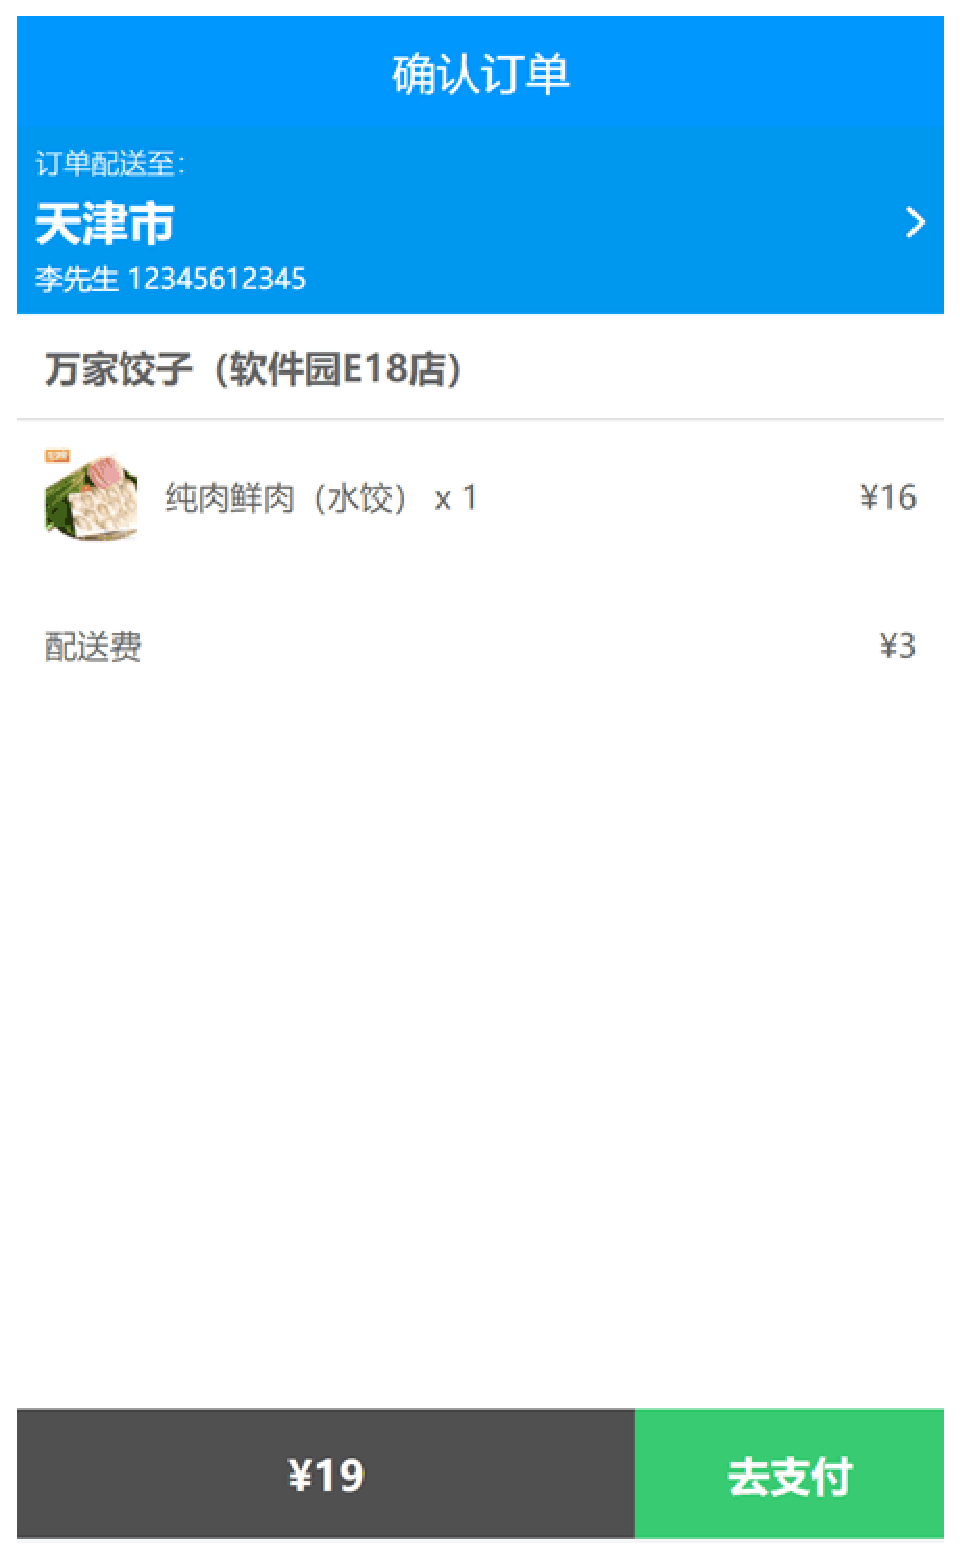
\includegraphics[width=0.6\textwidth]{order}
    \caption{确认订单}\label{fig:ord}
    \vspace{\baselineskip}
    \end{figure}

\begin{verbatim}
确认订单页面中,在选择地址时发现该项目与实际不符合的情况:当切换地址时,该项目会将地址改变,而地址下的姓名和电话仍为userName和userId,实际情况应为deliveryaddress表中的contactName和contactTel.
因此在此处做出修改:
当该用户的deliveryaddress为空时,则此处的姓名和电话为userName和userId,当该用户的deliveryaddress不为空时,此处的姓名和电话为contactName和contactTel。
\end{verbatim}    

\item
\begin{figure}[htbp]
    \centering
    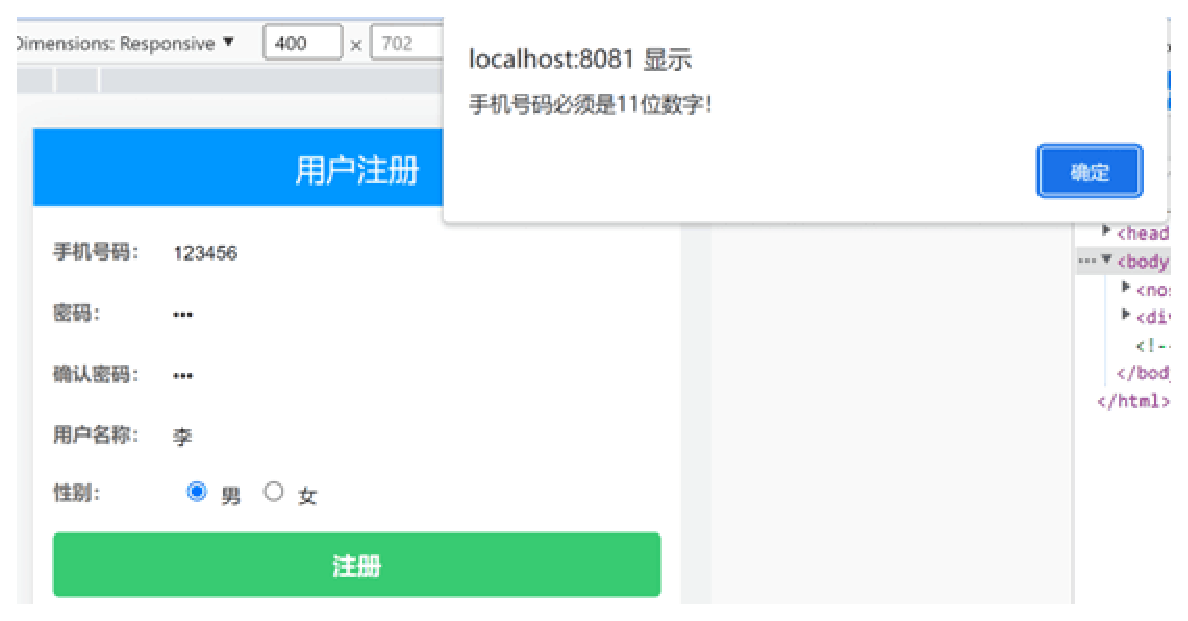
\includegraphics[width=0.8\textwidth]{11}
    \caption{注册页面}\label{fig:xml}
    \vspace{\baselineskip}
    \end{figure}

\begin{verbatim}
用户注册页面中,由于正确的手机号码应为11位数字。
因此在此处做出修改:
当输入的手机号码不为11位时,弹出提示框“手机号码必须是11位数字”    
\end{verbatim}

\begin{figure}[htbp]
\centering

\includegraphics[width=0.8\textwidth]{pay}
\caption{我的订单}\label{fig:xml}
\vspace{\baselineskip}
\end{figure}

\item
\begin{verbatim}
在我的订单页面,由于此页面去支付未设置功能。
因此在此处做出修改:
点击去支付按钮,跳转到支付页面。
      
\end{verbatim}


\end{enumerate}